\section{Feature Embedding Visualization}
\label{sec:visualize}

We investigate the effect of instance normalization on fine-grained control in sketch-based photorealistic image generation by designing a set of hand-drawn sketches and visualizing the feature embedding.
\dlt{In Sec.~\ref{sec:pix2pixhd}, we review our baseline method pix2pixHD.
In Sec.~\ref{sec:visualize}, we visualize the feature embedding from hand-drawn sketches by the generator of pix2pixHD, and analyze the visualization results to investigate the effect of instance normalization. 
Based on the analysis, we introduce our design on the generator network for sketch-based face generation in Sec.~\ref{sec:network}.
}
%\subsection{The pix2pixHD Baseline}\label{sec:pix2pixhd}
We employ Pix2pixHD~\cite{pix2pixhd} as our baseline model.
Its generator $G$ is composed of two sub-networks, a global generator network $G_1$ and a local enhance network $G_2$. 
$G_1$ is used to generate a base image, then $G_2$ is used to increase the image resolution with texture details. 
In order to distinguish real and generated images with high resolution, pix2pixHD uses a multi-scale discriminator, which is composed of three discriminators $D_1$, $D_2$, and $D_3$ in three scales, to preserve both global and local information. 
The loss function of this model is composed of three parts: adversarial loss $L_{GAN}(G,D_k)$, feature matching loss $L_{FM}(G,D_k)$, and VGG perceptual loss $L_{VGG}(G)$. The full objective is:
\begin{equation}
\begin{split}
&\underset{G}{\min}\Bigg(\bigg(\underset{D_1,D_2,D_3}{\max} \sum_{k=1,2,3}{L_{GAN}\big(G,D_k\big)}\bigg)+  \\
&\lambda \bigg(\frac{1}{3}\sum_{k=1,2,3}{L_{FM}\big(G,D_k\big)}+L_{VGG}{\big(G\big)}\bigg)\Bigg),
\end{split}
\end{equation}
\noindent
where $\lambda$ balances the three loss terms.


Pix2pixHD can be applied to sketch-based face generation when trained using pairs of synthesized contours and photos. 
We developed an interactive system to support users to create face images by sketching. 
However, when an user changes the shape of a local part, pix2pixHD tends to change the entire image globally, as shown in Fig.~\ref{fig:problem-in}.
Therefore, we investigate the network architecture and feature embedding through a comprehensive experiment.

\begin{figure}
	\centering
	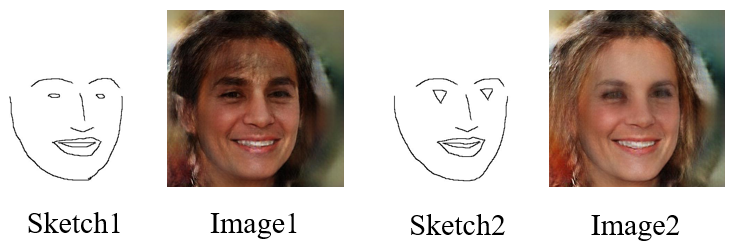
\includegraphics[width=\columnwidth]{figures/prob-in-pix2pixHD.png}
	\caption{Pix2pixHD fails to support fine-grained control on the synthesized images when the input sketch changes locally.}
	\label{fig:problem-in}
\end{figure}


\begin{figure}
	\centering
	\begin{subfigure}[b]{0.2\textwidth}	
		\centering
		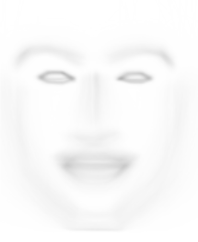
\includegraphics[width=0.13\textheight]{average_face.png}
		\caption{ }
		\label{fig:average_face}
	\end{subfigure}	
	\hfill
	\begin{subfigure}[b]{0.2\textwidth}
		\centering
		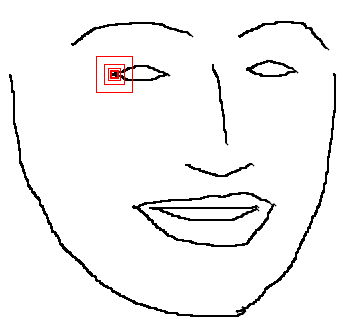
\includegraphics[width=0.15\textheight]{receptive_field.png}
		\caption{ }
		\label{fig:receptive}
	\end{subfigure}	
	
	\caption{(a) The average face of all the synthesized contours from the face photos. (b) The receptive fields of corresponding left eye corner points in the feature maps of $L_0\sim L_4$.}
\end{figure}





%\subsection{Feature Visualization}\label{sec:visualize}

 
In order to analyze how the image translation model extracts the face shape features consistent with the user's intention for the hand-drawn sketches that typically contain little details and geometric deformation, we collect 11 groups of sketches with changes in a specific area in each group. It contains 198 sketches of resolution $512\times512$. 
Note that all synthetic face contours in the training set are globally aligned.
We compute an average face (Fig.~\ref{fig:average_face}) and show it in the drawing panel as reference when collecting sketches. 
%
Fig.~\ref{fig:hand_drawn_contours} shows some examples of the 11 groups of sketches, denoted as $G_1,\ldots,G_{11}$.

We refer to the first five layers of the global generator of pix2pixHD as $L_0,\ldots,L_4$. 
With a sketch fed into the generator, five groups of feature maps can be obtained from $L_0$ to $L_4$.
For each point in a layer, we can extract a $k$-dimensional feature vector, where $k$ is the channel number of the feature maps in that layer.
We select the corner of the left eye for visual analysis. 
The five feature vectors are denoted as $\boldsymbol{v}_0,\boldsymbol{v}_1,\boldsymbol{v}_2,\boldsymbol{v}_3,\boldsymbol{v}_4$ in dimensions of 48, 96, 192, 384 and 768, respectively. 
%The coordinates of the corresponding points on the five feature maps are (170, 250), (85, 125), (43, 63), (22, 32) and (11, 16). 
The receptive fields of the five vectors are $7\times7$, $9\times9$, $13\times13$, $21\times21$, and $37\times37$ respectively on the input sketch, as shown in Fig.~\ref{fig:receptive}. 

%\textcolor{blue}{
%We get the five feature vectors of pix2pixHD generator called $\boldsymbol{v}_0^{'},\ldots,\boldsymbol{v}_4^{'}$ in the same way.}


%\paragraph{Visualization with PCA.} 
%\noindent\textbf{Visualization with PCA.} 
Principal component analysis~(PCA)~\cite{pca} is a widely-used dimension reduction method and retains the statistic characteristics of data in high dimensional space. 
We employ PCA on $\boldsymbol{v}_0,\ldots, \boldsymbol{v}_4$ to map the high-dimensional vectors into 2D vectors and plot them in a 2D space. 
Fig.~\ref{fig:pca_0} show the visualization results with PCA on $\boldsymbol{v}_0,\ldots,\boldsymbol{v}_4$. 
%
In $G_{1}$, all the sketches share the same eye shape but with different hair styles. They are supposed to have the same feature embedding for the left eye corner at the early convolutional layers. However, as shown in Fig.~\ref{fig:pca_0}, the feature vectors scatter across a wide range (red numbers). 
Similarly, though the eye strokes do not change in the sketches of the same group, the feature embedding of $G_2$ (orange), $G_3$ (lime), $G_4$ (blue), $G_8$ (olive), $G_9$ (green), $G_{10}$ (purple), and $G_{11}$ (teal) scatter a lot.
This indicates that the instance normalization in each layer takes the sketch information outside of its corresponding receptive field into account and then affects the feature embedding of a local region. 
By comparing visualization results of $\boldsymbol{v}_0\sim\boldsymbol{v}_4$ comprehensively, we find that the feature vectors belonging to the groups without eye changes, such as $G_1$, $G_2$, $G_3$, $G_4$, $G_8$, $G_9$, $G_{10}$, and $G_{11}$, distribute more and more dispersedly within each group from layer 1 to layer 4, indicating that with more instance normalization, changing other parts on the input sketch has more and more influence on the local feature embedding, resulting in an awful change of eyes in the generated images.
Consequently, we modify the normalization in the generator of pix2pixHD to keep local shape details. 

\begin{figure}[htbp]
	\centering
	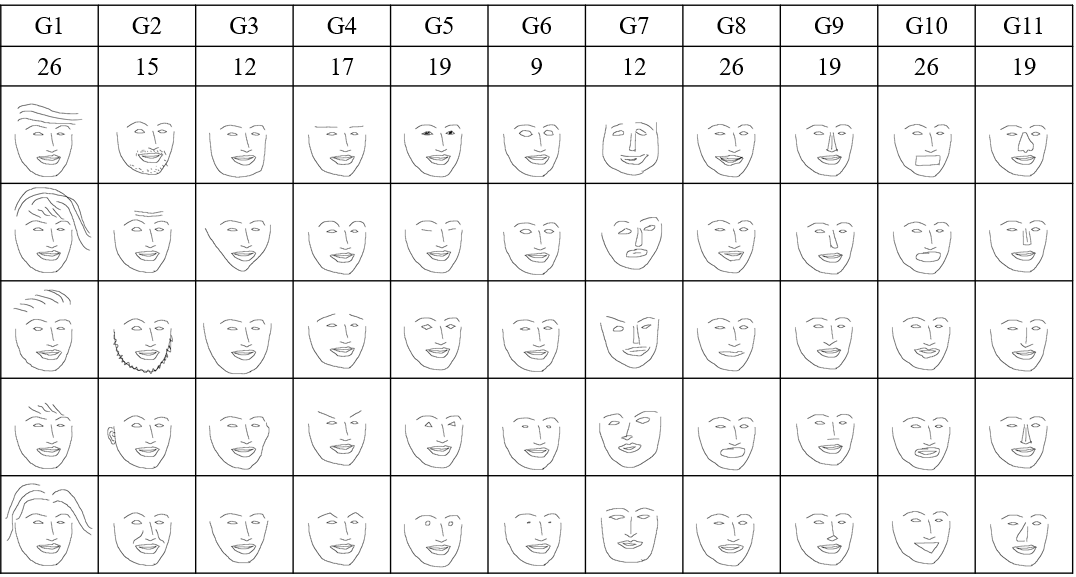
\includegraphics[width=0.5\textwidth]{hand_drawn_sketches.png}
	\caption{11 groups of hand-drawn sketches with specific changes at each group. $G_1$: Add hair; $G_2$: Add new attributes, such as whiskers, wrinkles, and ears; $G_3$: Face shape change; $G_4$: Eyebrow change; $G_5$: Eye shape change; $G_6$: Eye size change; $G_7$: Graffiti-drawn; $G_8$: Mouth shape change; $G_9$: Nose shape change; $G_{10}$: Mouth shape change with the same eyes as $G_{9}$; $G_{11}$: Nose shape change with the same eyes as $G_{8}$. The second row lists the number of sketches in each group.
		%Specifically, there is no correlation between G7 and the other 10 groups. Except G7, in the sketches of other groups, only a particular area or attribute is modified while the rest sketches in this group remain the same. While sketches in G8 and G11 have the same eyes, sketches in G9 and G10 have the same eyes, the eye shapes in other groups are different.
	}
	\label{fig:hand_drawn_contours}
\end{figure}


\begin{figure}[htb]
	\centering
	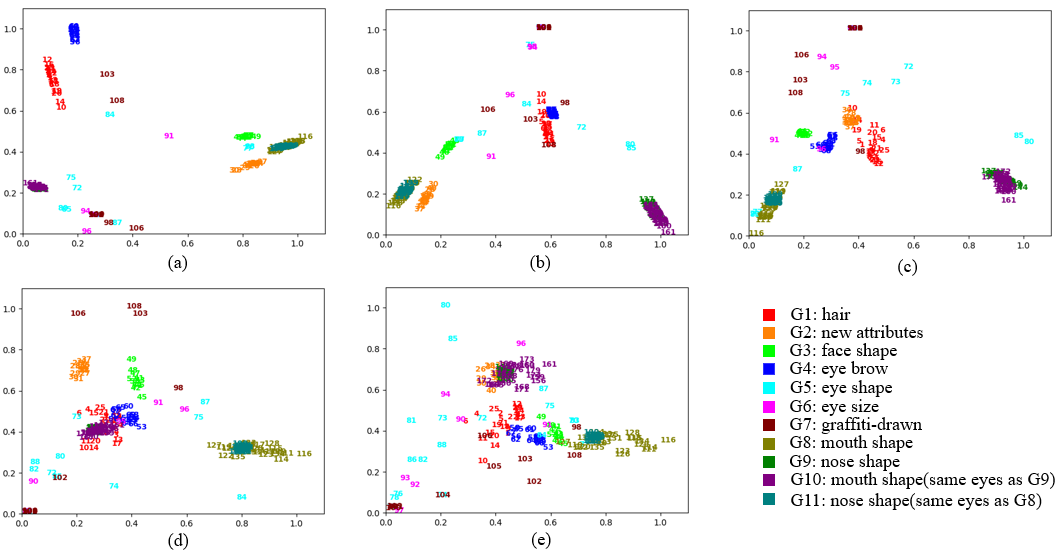
\includegraphics[width=0.5 \textwidth]{pca_0.png}
	\caption{Visualization of feature embedding $\boldsymbol{v}_0\sim\boldsymbol{v}_4$ in the first five layers of the global generator of pix2pixHD at the left eye corner for 11 groups of sketches.  }
	\label{fig:pca_0}
\end{figure}      

\begin{figure}[htb]
	\centering
	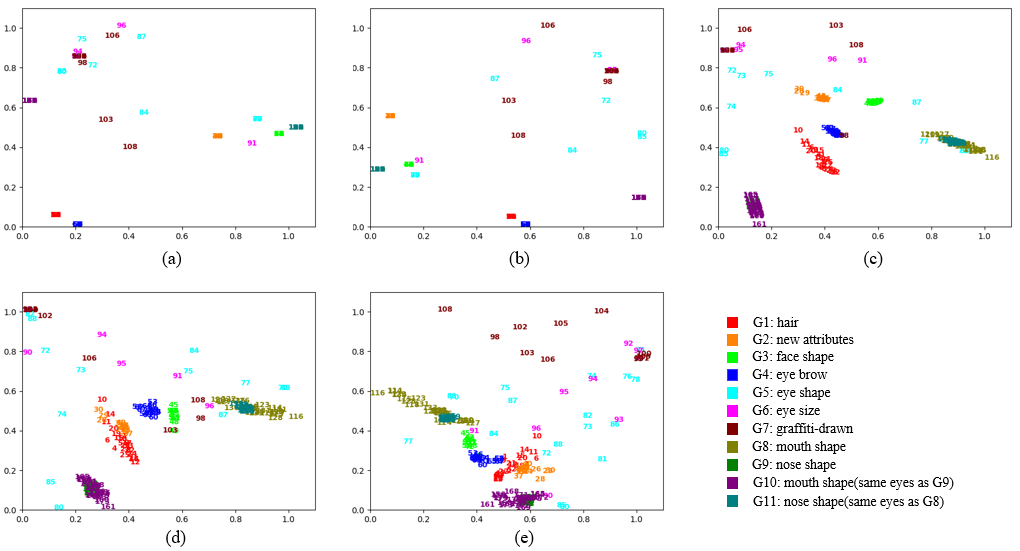
\includegraphics[width=0.5 \textwidth]{pca_1.png}
	\caption{Visualization of  $\boldsymbol{v}_0^{'}\sim\boldsymbol{v}_4^{'}$ in the first five layers of our generator at the left eye corner for 11 groups of sketches.}
	\label{fig:pca_1}
\end{figure}


\section{Our Network Design}\label{sec:network}
%
 
With instance normalization in the baseline generator, the activation of convolutional output is normalized in a channel-wise manner and then modulated with unified scale and bias within each channel. 
This operation, to a certain extent, leads to a negative effect that a local change in the input sketch broadcasts globally, resulting in a degraded capacity of fine-grained control on the generated images.
However, the vanishing gradient or exploding gradient problem is bound to emerge when the instance normalization layers in the feature embedding stage of the generator is abandoned, making the training process difficult to converge. 
 
Based on the consideration above, we only remove the first two instance normalization layers in the global generator of pix2pixHD and keep the rest the same as pix2pixHD. 
The architecture of our generator is shown in Fig.~\ref{fig:our_generator}. 
%It operates at a resolution of 512×512. 
It consists of four components: a convolutional front-end without normalization $G_F$, a down-sampled convolutional mid-end $G_M$, a set of residual blocks $G_R$, and a transposed convolutional back-end $G_B$.  
$G_F$, which is composed of two un-normalized convolution and activation layers, embeds local shape information of the input sketch.
In other words, the local shape information of the sketch can flow through the network without spatially broadcasting, thus effectively supports fine-grained control on generated images. 

\begin{figure}[htbp]
	\centering
	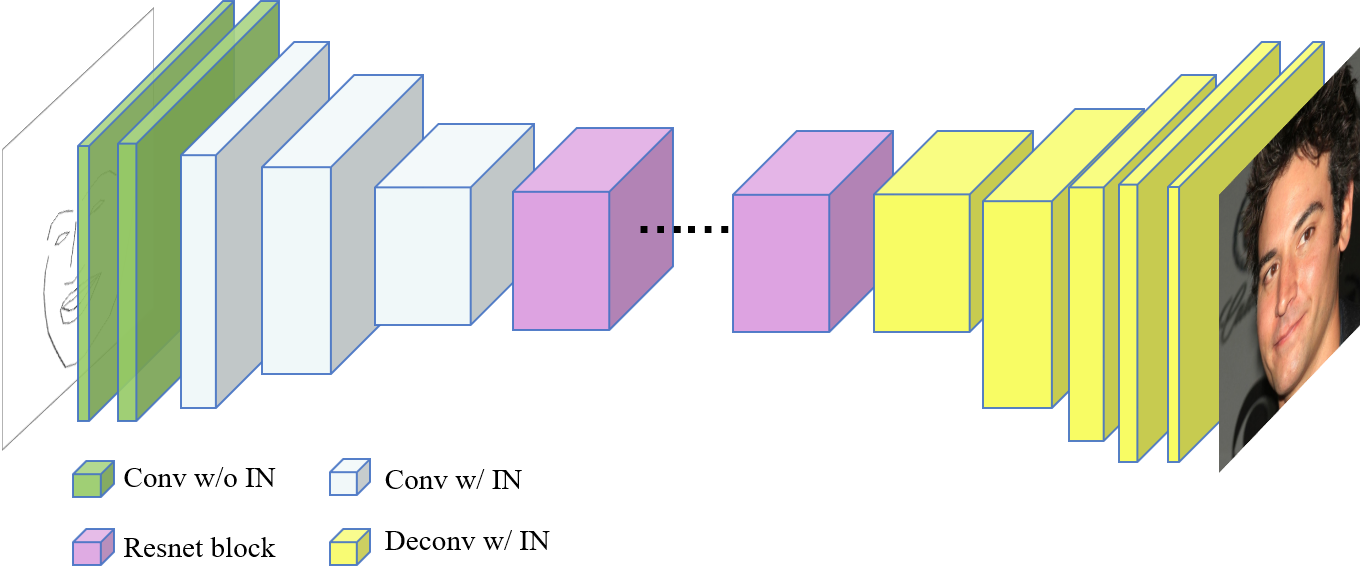
\includegraphics[width=\columnwidth]{our_model_G.png}
	\caption{Network architecture of our generator. }
	\label{fig:our_generator}
\end{figure}

\dlt{
We use the same three-scale discriminator with pix2pixHD. 
Each discriminator is built on the PatchGAN~\cite{pix2pix} architecture. 
At each scale, the input sketch is concatenated with the corresponding face images, resized and fed into the corresponding discriminator.
}

%To evaluate the superiority of our proposed method at the level of feature embedding, we conducted the visual analysis in the same way as described in Sec.~\ref{sec:visualize}.
We refer to the five feature vectors in our generator as $\boldsymbol{v}_0^{'},\boldsymbol{v}_1^{'},\boldsymbol{v}_2^{'},\boldsymbol{v}_3^{'},\boldsymbol{v}_4^{'}$.
%
Fig.~\ref{fig:pca_1} (a)(b) demonstrate the results of PCA visualization on $\boldsymbol{v}_0^{'}$ and $\boldsymbol{v}_1^{'}$. 
The feature vectors from $G_1$, $G_2$, $G_3$, and $G_4$ are located at the same point in each group. The feature vectors from G8 and G11 are gathered on the same point since these two groups share the same eye shape, so do the feature vectors from $G_9$ and $G_{10}$.
On the contrary, the feature vectors from $G_5$, $G_6$, and $G_7$ distribute dispersedly, indicating that after the removal of instance normalization in the first two layers of generator, the feature embedding of the left eye corner conforms with the local shape of the sketches inside of the corresponding receptive fields. 

%The sketch change within the receptive field will influence the embedded features of the corresponding point but not outside of the receptive field.

%\begin{figure*}[htb]
%	\centering
%	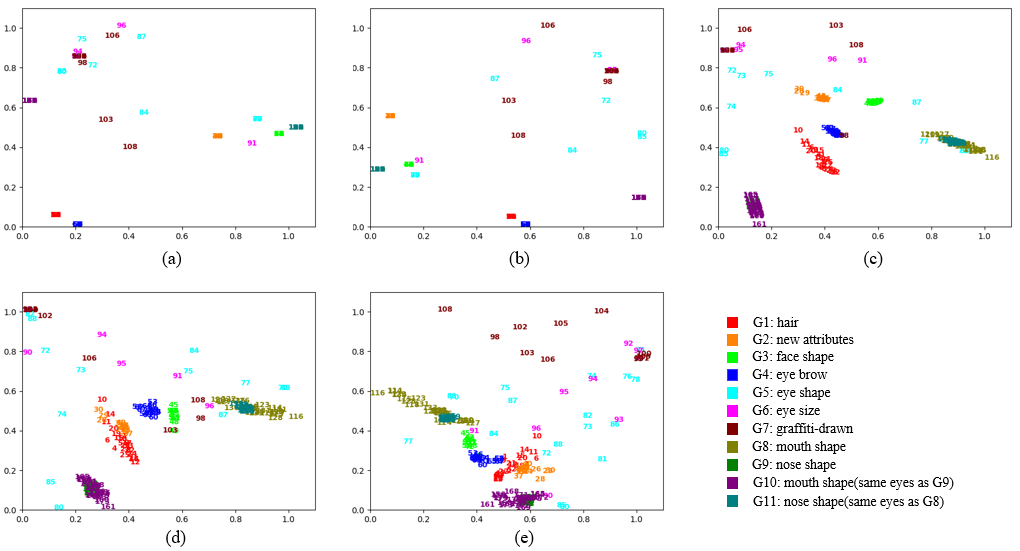
\includegraphics[width=0.9 \textwidth]{pca_1.png}
%	\caption{Visualization of feature embedding $\boldsymbol{v}_0^{'}\sim\boldsymbol{v}_4^{'}$ in the first five layers of our generator for the left eye corner for 11 groups of sketches.}
%	\label{fig:pca_1}
%\end{figure*}

We visualize the feature embedding of $\boldsymbol{v}_2^{'},\boldsymbol{v}^{'}_3, \boldsymbol{v}_4^{'}$ in Fig.~\ref{fig:pca_1} (c) (d) (e). 
Compare with the PCA visualization results of $\boldsymbol{v}_2,\boldsymbol{v}_3,\boldsymbol{v}_4$ in 
Fig.~\ref{fig:pca_0} (c) (d) (e), the $\boldsymbol{v}_2, \boldsymbol{v}_3, \boldsymbol{v}_4$ belonging to groups without eye shape change, such as $G_1$, $G_2$, $G_3$, $G_4$, $G_8$, $G_9$, $G_{10}$, and $G_{11}$, have a bigger in-class distance compared with $\boldsymbol{v}_2^{'}, \boldsymbol{v}_3^{'}, \boldsymbol{v}_4^{'}$. 
This indicates that the removal of the first two instance normalization layers in pix2pixHD generator can better extract the low-level features of the input sketch and keep local shape information. 
%The improvement on generator network can effectively alleviate the issue that changing one part of the sketch influences the other parts of the generated image. 
Therefore, our network better supports fine-grained control and enhances texture details on the generated images.

